\section{Markov Decision Processes}
\begin{framed}
    A \textbf{Markov decision process} is specified by a set of \textbf{states} $\sX \defeq \{1, \dots, n\}$; a set of \textbf{actions} $\sA \defeq \{1, \dots, m\}$; \textbf{transition probabilities} ${p(x' \mid x, a) \defeq \Pr{X_{t+1} = x' \mid X_t = x, A_t = a}}$; a \textbf{reward function} $r : X \times A \to \R$ which maps the current state $x$ and an action $a$ to some \textbf{reward}. \\
\end{framed}
$r$ induces a sequence of rewards: $R_t \defeq r(X_t, A_t)$.
\begin{framed}
    A \textbf{policy} is a function that maps each state $x \in \sX$ to a probability distribution over the actions. That is, for any $t > 0$: \\
    $\pi(a \mid x) \defeq \Pr{A_t = a \mid X_t = x}$.
\end{framed}
A policy induces a MC $(X_t^\pi)_{t\in\Nat_0}$: $p^\pi(x' \mid x) \defeq \Pr{X_{t+1}^\pi = x' \mid X_t^\pi = x} = \sum_{a \in \sA} \pi(a \mid x) p(x' \mid x, a)$.\\
The \textbf{discounted payoff} from time $t$ given discount factor $\gamma \in [0, 1)$ is\\
 $G_t \defeq \sum_{m=0}^\infty \gamma^m R_{t+m}$
\begin{framed}
    The \textbf{state value function}: $\E[\pi]{\cdot} \defeq \E[(X_t^\pi)_{t\in\Nat_0}]{\cdot}$ measures the average discounted payoff from time $t$ starting from state $x \in \sX$.
\end{framed}
\begin{framed}
    The \textbf{state-action value function q}: \\
    $\q[\pi]{x}{a}[t] \defeq \E[\pi]{G_t \mid X_t = x, A_t = a}$ \\
    $ = r(x, a) + \gamma \sum_{x' \in \sX} p(x' \mid x, a) \cdot \v[\pi]{x'}[t+1]$ measures the average discounted payoff from time $t$ starting from state $x \in \sX$ and with playing action $a \in \sA$.
\end{framed}
\begin{framed}
    \textbf{Bellman Expectation Equation}\\
    $\v[\pi]{x} = r(x, \pi(x)) + \gamma \E[x' \mid x, \pi(x)]{\v[\pi]{x'}}$ \\
    For stochastic policy: $\v[\pi]{x} = \E[a \sim \pi(x)]{\q[\pi]{x}{a}}$ \\
    $\q[\pi]{x}{a} = r(x, a) + \gamma \E*[x' \mid x, a]{\E[a' \sim \pi(x')]{\q[\pi]{x'}{a'}}}$.\\
    For deterministic: $\v[\pi]{x} = \q[\pi]{x}{\pi(x)}$.
\end{framed}
Can be used to find $\fnv[\pi]$ given policy $\pi$, by solving linear system of equations in cubic time in the size of the state space. Can also be solved using fixed point iteration: $\mB^\pi \vv \defeq \vr^\pi + \gamma \mP^\pi \vv$.
\begin{framed}
    \textbf{Greedy policies} \\
    Greedy w.r.t. to state-action value function $\fnq$: is $\pi_{\fnq}(x) \defeq \argmax_{a \in \sA} \q{x}{a}$;\\
    Greedy w.r.t. a state value function $\fnv$ is: \\
    $\pi_{\fnv}(x) \defeq \argmax_{a \in \sA} r(x, a)$ \\
    $ \quad+ \gamma \sum_{x' \in \sX} p(x' \mid x, a) \cdot \v{x'}$.
    \vspace{2mm}
\end{framed}
\begin{framed}
    \textbf{Bellman's Theorem}: A policy $\pis$ is optimal iff it is greedy with respect to its own value function. In other words, $\pis$ is optimal iff $\pis(x)$ is a distribution over the set $\argmax_{a \in \sA} \q*{x}{a}$.
\end{framed}
If for every state there is a unique action that maximizes $q$, $\pis(x) = \argmax_{a \in \sA} \q*{x}{a}$ is deterministic and unique.
% 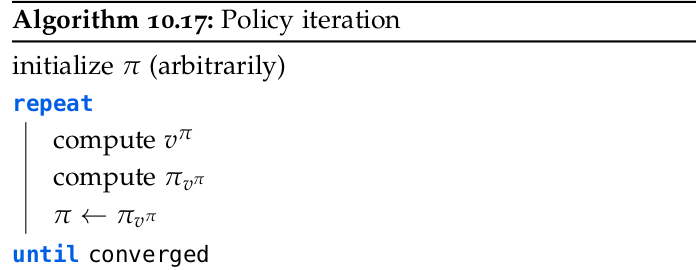
\includegraphics[width=0.9\linewidth]{images/Policy_Iteration.png} \\
\begin{framed}
    \textbf{Policy Iteration} \\
    1. Initialize $\pi_0$ arbitrarily. \\
    2. Compute $\fnv[\pi_k]$ as $\mB^{\pi_k} \vv = \vv$ (iter. or LSE). \\
    3. Compute $\pi_{k+1} = \pi_{(\fnv[\pi_k])}$ greedily. \\
    4. Repeat steps 2 and 3 until $\pi_k = \pi_{k+1}$.
\end{framed}
Finite MDP: Policy it. converges monot. to an optimal $\pi$ in $\mathcal{O}(\card{\sX}^2 \card{\sA} / (1 - \gamma))$ steps.
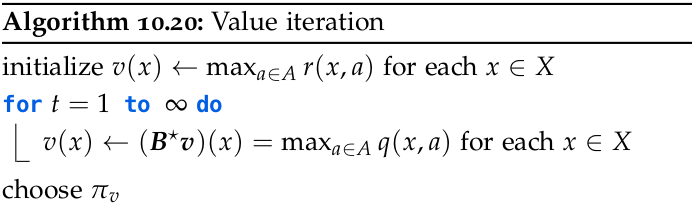
\includegraphics[width=0.9\linewidth]{images/Value_Iteration.png}
VI. converges to an $\epsilon$-optimal policy, as $\fnv[\star]$ and $\fnq[\star]$ are fixed-points of the Bellman update $\mBs$.
\begin{framed}
    A \textbf{Partially observable MDP (POMDP)} is a Markov process, with a set of supplementary \textbf{observations} $\sY$, and \textbf{observation probabilities} $o(y \mid x) \defeq \Pr{Y_t = y \mid X_t = x}$.
\end{framed}
Reduce POMDP to MDP with enlarged state space. We consider MDP whose states are \textbf{beliefs}: $b_t(x) \defeq \Pr{X_t = x \mid y_{1:t}, a_{1:t-1}}$. Keeping track of how beliefs change over time is \textbf{Bayesian filtering}: Given a prior belief $b_t$, an action taken $a_t$, and a new observation $y_{t+1}$, the belief state can be updated as: $b_{t+1}(x) = \Pr{X_{t+1} = x \mid y_{1:t+1}, a_{1:t}} = \frac{1}{Z} o(y_{t+1} \mid x) \sum_{x' \in \sX} p(x \mid x', a_t) b_t(x')$, where $Z \defeq \sum_{x \in \sX} o(y_{t+1} \mid x) \sum_{x' \in \sX} p(x \mid x', a_t) b_t(x')$.
The sequence of belief-states defines the sequence of RVs $(B_t)_{t\in\Nat_0}$:$ B_t \defeq X_t \mid y_{1:t}, a_{1:t-1}$, where the (state--)space of all beliefs is the (infinite) space of all probability distributions over $\sX$: $\spB \defeq \Delta^{\sX} \defeq \braces*{\vb \in \R^{\card{\sX}} : \vb \geq \vzero, \textstyle\sum_{i=1}^{\card{\sX}} \vb(i) = 1}$.
\begin{framed}
    Given a POMDP, the corresponding \textbf{Belief-state MDP} is an MDP specified by \textbf{belief space} $\spB \defeq \Delta^{\sX}$ depending on \textbf{hidden states} $\sX$; the set of \textbf{actions} $\sA$; \textbf{transition probabilities} $\tau(b' \mid b, a) \defeq \Pr{B_{t+1} = b' \mid B_t = b, A_t = a}$; and \textbf{rewards} $\rho(b, a) \defeq \E[x \sim b]{r(x, a)} = \sum_{x \in \sX} b(x) r(x, a)$.
\end{framed}
Have: $\tau(b_{t+1} \mid b_t, a_t) = \Pr{b_{t+1} \mid b_t, a_t} = \sum_{y_{t+1} \in \sY} \Pr{b_{t+1} \mid b_t, a_t, y_{t+1}} \Pr{y_{t+1} \mid b_t, a_t}$. We also set: $\Pr{b_{t+1} \mid b_t, a_t, y_{t+1}} = 1$ iff $b_{t+1}$ matches the belief update given $b_t, a_t$, and $y_{t+1}$, and 0 else. Finally the likelihood is: $\Pr{y_{t+1} \mid b_t, a_t} = \E[x \sim b_t]{\E[x' \mid x, a_t]{\Pr{y_{t+1} \mid X_{t+1} = x'}}} = \sum_{x \in \sX} b_t(x) \sum_{x' \in \sX} p(x' \mid x, a_t) \cdot o(y_{t+1} \mid x')$.